% CYBEL — ROSCon Korea 2027 companion paper (max 8 pages, IEEE two-column)
% Build: pdflatex main && bibtex main && pdflatex main && pdflatex main
\documentclass[conference]{IEEEtran}

\usepackage[T1]{fontenc}
\usepackage[utf8]{inputenc}
\usepackage{cite}
\usepackage{amsmath,amssymb}
\usepackage{graphicx}
\usepackage{booktabs}
\usepackage{url}
\usepackage{hyperref}
\usepackage{xcolor}
\usepackage{enumitem}
\usepackage{tikz}
\usetikzlibrary{arrows.meta,positioning,fit,calc}

\hypersetup{colorlinks=true,linkcolor=black,citecolor=black,urlcolor=blue!50!black}

%% Tighten vertical space for 8-page limit
\setlength{\textfloatsep}{8pt plus 2pt minus 2pt}
\setlength{\floatsep}{6pt plus 2pt minus 2pt}
\setlength{\intextsep}{6pt plus 2pt minus 2pt}
\setlist{nosep,leftmargin=*}

\newcommand{\ros}{\textsc{ros}}
\newcommand{\rosbridge}{\textsc{rosbridge}}
\newcommand{\rosapi}{\texttt{rosapi}}
\newcommand{\cybel}{\textsc{Cybel}}

\begin{document}

\title{Non-Destructive Reverse Engineering of a Closed Android--\ros{} Service Robot:\\
Open \rosbridge{} Integration and Edge Conversational Stack Without Vendor Support}

\author{
\IEEEauthorblockN{Claudia LUSAMOTE KIMFUTA}
\IEEEauthorblockA{HESTIM Engineering \& Business School\\
Email: \texttt{clusamote@gmail.com}}
\and
\IEEEauthorblockN{Dr. Sridath Tula}
\IEEEauthorblockA{HESTIM Engineering \& Business School\\
Supervisor}
}

\maketitle

\begin{abstract}

Commercial service robots often ship with proprietary Android applications and undisclosed communication protocols, preventing customization of reception flows, guided tours, and conversational assistants.
We present \cybel{}, an open edge platform built by \emph{non-destructive reverse engineering} of the CIOT TY1251D-03195 reception robot a dual-processor system combining a \ros{} navigation chassis and an Android~7.1 head without manufacturer documentation or support.
Our seven-phase methodology combines network mapping, \rosbridge{}/\rosapi{} introspection, static APK analysis (JADX)~\cite{cybel_architecture}, passive MQTT observation, and field validation using rule \textbf{H4}: a successful \rosbridge{} transport acknowledgment does not guarantee motor execution.
We document reconstructed teleoperation (\texttt{/cmd\_vel\_mux/input/teleop}), autonomous navigation (\texttt{/navi\_goal} vs.\ POI chain \texttt{/tag\_manager/navi}), and an edge conversational layer local knowledge engine, Android TTS bridge, guided tour orchestration replacing the vendor welcome application.
A hybrid strategy reusing POIs from the manufacturer Deployment Tool (Sentrymove) improves navigation reliability over coordinate-only goals.
Field results show ${<}100$\,ms local API latency, ${\sim}90\%$ \rosbridge{} session reliability, and an autonomous visitor kiosk on Termux.

\end{abstract}

\begin{IEEEkeywords}
Service robotics, reverse engineering, \ros{}, \rosbridge{}, embedded Android, human-robot interaction, edge computing, text-to-speech
\end{IEEEkeywords}

%==============================================================================
\section{Introduction}
%==============================================================================

Mobile reception robots integrate mature SLAM and motion planning with touchscreen and speech interfaces, yet remain software black boxes: no public SDK, no message schemas, and often mandatory vendor cloud services.
For research labs and training institutions, this closure blocks custom visit paths, domain-specific knowledge bases, and open conversational agents.

We address the question: \emph{How can a third-party command and interaction platform match or exceed a proprietary Android-\ros{} welcome application when no official interface documentation exists?}
Sub-problems include discovering network entry points, reconstructing message formats, validating causal command effects, rebuilding speech when \ros{} exposes no TTS channel, and operating on closed robot Wi-Fi without guaranteed Internet.

\textbf{Contributions} (project \cybel{}, HESTIM 2026):
\begin{enumerate}[label=\textbf{C\arabic*.},leftmargin=1.4em]
\item A reproducible seven-phase non-destructive reverse-engineering pipeline for closed vendor robots.
\item Documented \rosbridge{} v2 reconstruction for teleop, POI/coordinate navigation, and telemetry.
\item Edge-first architecture: interchangeable \texttt{MockRobot}/\texttt{RealRobot} SDK, dual PC/Termux backend, autonomous WebView kiosk.
\item Empirical TTS resolution via a minimal Android broadcast bridge when \ros{}, HTTP, and MQTT fail.
\item Open conversational layer (local FAQ + robot actions), extensible to LLMs without vendor cloud.
\item Hybrid Sentrymove POI reuse strategy improving field navigation over raw coordinates.
\end{enumerate}

\textbf{Scope.} This paper focuses on protocol discovery and open-stack integration; LLM chatbots are architected but not yet deployed.
The codebase and exploration scripts are maintained as reproducible artifacts.

%==============================================================================
\section{Robot Platform and Network Topology}
%==============================================================================

\subsection{Dual-processor hardware}

The CIOT TY1251D-03195 combines:
\begin{itemize}
\item \textbf{Chassis:} Linux + \ros{} (Noetic/Melodic), SLAM, \texttt{move\_base}, LiDAR/RGBD, \rosbridge{}, MQTT broker.
\item \textbf{Head:} Android~7.1 (RK3399, 2\,GB RAM) - 15.6'' touchscreen, cameras, speakers, vendor apps.
\end{itemize}

\cybel{} never obtains shell access on the chassis (SSH locked; brute-force triggers lockout).
Usable channels: WebSocket \rosbridge{} on port~9090 and MQTT on 1883 (observation only).

\subsection{Triple network segment}

Mapping revealed three distinct segments (Fig.~\ref{fig:network}):

\begin{figure}[!t]
\centering
\resizebox{\columnwidth}{!}{%
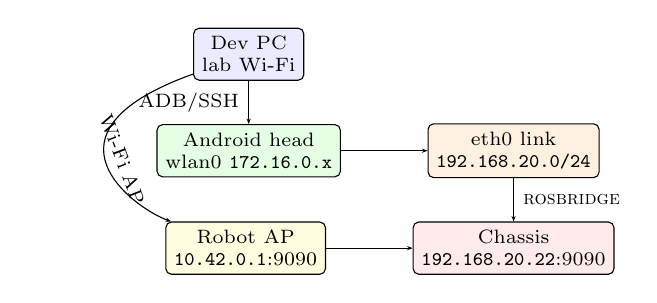
\begin{tikzpicture}[
  node distance=0.55cm and 0.4cm,
  box/.style={draw, rounded corners=2pt, align=center, font=\scriptsize, inner sep=3pt},
  arr/.style={-{Stealth[length=2pt]}, font=\tiny}
]
  \node[box, fill=blue!8] (pc) {Dev PC\\{\scriptsize lab Wi-Fi}};
  \node[box, fill=green!10, below=of pc] (head) {Android head\\{\scriptsize wlan0 \texttt{172.16.0.x}}};
  \node[box, fill=orange!12, right=1.1cm of head] (eth) {eth0 link\\{\scriptsize \texttt{192.168.20.0/24}}};
  \node[box, fill=red!8, below=of eth] (ch) {Chassis\\{\scriptsize \texttt{192.168.20.22}:9090}};
  \node[box, fill=yellow!12, left=1.1cm of ch] (wifi) {Robot AP\\{\scriptsize \texttt{10.42.0.1}:9090}};

  \draw[arr] (pc) -- node[left]{\scriptsize ADB/SSH} (head);
  \draw[arr] (head) -- (eth);
  \draw[arr] (eth) -- node[right]{\scriptsize \rosbridge{}} (ch);
  \draw[arr] (pc) .. controls +(-2.8,-1) and +(-1.4,0.5) .. node[above,sloped]{\scriptsize Wi-Fi AP} (wifi);
  \draw[arr] (wifi) -- (ch);
\end{tikzpicture}%
}
\caption{Network topology. Termux on the tablet uses \texttt{192.168.20.22}; confusing head DHCP IP with chassis IP causes silent failures.}
\label{fig:network}
\end{figure}

\begin{itemize}
\item \textbf{Robot AP} (\texttt{TY1251D-03195}): chassis at \texttt{10.42.0.1:9090}.
\item \textbf{Internal eth0:} head \texttt{192.168.20.1} $\leftrightarrow$ chassis \texttt{192.168.20.22:9090}, preferred path from Termux.
\item \textbf{Lab Wi-Fi:} head \texttt{172.16.0.x} (DHCP); PC uses ADB for deployment.
\end{itemize}

Vendor packages identified via ADB: \texttt{com.ciot.welcomepatrol} (welcome UI), \texttt{com.ciot.sentrymove} (Deployment Tool), shared library \texttt{selfchassislibrary} treated as \emph{de facto} protocol specification after JADX audit.

%==============================================================================
\section{Reverse Engineering Methodology}
%==============================================================================

\subsection{Guiding principles}

\begin{enumerate}[label=\textbf{P\arabic*.},leftmargin=1.4em]
\item Observe before publishing (passive MQTT/\rosbridge{} first).
\item Verify real effects  rule \textbf{H4}: after teleop publish, \texttt{/robot\_pose} must change.
\item Triangulate network traces, \rosapi{}, decompiled APK, and field logs.
\item Remain non-destructive: no firmware flash, no chassis root.
\item Mock-first development before \texttt{RealRobot} integration.
\end{enumerate}

\subsection{Seven-phase pipeline}

Table~\ref{tab:re-phases} summarizes the pipeline; each hypothesis follows \emph{observe $\rightarrow$ isolated script $\rightarrow$ telemetry check $\rightarrow$ SDK integration or documented rejection}.

\begin{table}[!t]
\caption{Reverse-engineering phases and deliverables}
\label{tab:re-phases}
\centering
\scriptsize
\begin{tabular}{@{}clp{3.6cm}@{}}
\toprule
\textbf{\#} & \textbf{Phase} & \textbf{Key deliverable} \\
\midrule
1 & Network scan & Dual-IP map, ports 9090/1883 \\
2 & \ros{} observation & Topic/service inventory \\
3 & MQTT passive & No movement control via MQTT \\
4 & APK audit (JADX) & Topic parity vs.\ Sentrymove \\
5 & Wireshark & WebSocket JSON framing \\
6 & ADB / Termux & TTS bridge, edge backend \\
7 & Field validation & \texttt{phase0\_robot\_check.py} \\
\bottomrule
\end{tabular}
\end{table}

Rejected hypotheses (documented): legacy teleop topic \texttt{/mobile\_base/commands/velocity}; candidate TTS topics (\texttt{/play\_tts}, \texttt{/robot\_tts}); HTTP TTS on head ports 80/8080/8888; MQTT movement commands.

%==============================================================================
\section{\rosbridge{} Protocol Reconstruction}
%==============================================================================

\subsection{Transport and client}

\rosbridge{} v2 over WebSocket TCP~9090~\cite{crick2012rosbridge,rosbridge_suite}; JSON operations \texttt{subscribe}, \texttt{publish}, \texttt{advertise}, \texttt{call\_service}.
Our \texttt{RosbridgeClient} (\texttt{sdk/rosbridge.py}) uses three connection retries (20\,s timeout), 20\,s ping keepalive, and automatic reconnect.

\subsection{Teleoperation}

Manufacturer-confirmed topic:
\begin{center}
\texttt{/cmd\_vel\_mux/input/teleop} \quad (\texttt{geometry\_msgs/Twist})
\end{center}
Sequence: \texttt{advertise} then periodic \texttt{publish} (${\sim}10$\,Hz).
Sentrymove ramps linear velocity $\pm 0.025$/100\,ms with $\omega_z \times 0.8$ scaling.

\textbf{Gap E1:} early \cybel{} builds blocked teleop unless manual mode was active (\texttt{control\_state==30}); Sentrymove does not require this step.
\textbf{Fix:} auto-enable manual mode on first \texttt{move()}.

\subsection{Autonomous navigation}

Two modes coexist on the chassis:

\begin{table}[!t]
\caption{Navigation modes and prerequisites}
\label{tab:nav}
\centering
\scriptsize
\begin{tabular}{@{}lll@{}}
\toprule
\textbf{Mode} & \textbf{Mechanism} & \textbf{Gate} \\
\midrule
Coordinates & \texttt{/navi\_goal} & loc.\ ${\geq}60\%$, status 601 \\
Named POI & \texttt{/tag\_manager/navi} $\rightarrow$ \texttt{/poi} & POI in map \\
\bottomrule
\end{tabular}
\end{table}

\texttt{nav\_status} codes gate \cybel{} commands: 600 not localized, 601 ready, 602 navigating, 603 arrived, 604 error.
Cancellation chain: \texttt{/move\_base/cancel}, \texttt{/path\_follower/cancel}, \texttt{/poi\{command:stop\}}, zero velocity on mux.

\subsection{Telemetry throttling}

Subscriptions use \texttt{throttle\_rate} (ms): \texttt{/robot\_pose} 200 (${\sim}5$\,Hz), \texttt{/navi\_status} 500, LiDAR \texttt{/scan\_filter} 100 --- limiting \rosbridge{} saturation on constrained Wi-Fi.

%==============================================================================
\section{\cybel{} Software Architecture}
%==============================================================================

\subsection{Three-layer stack}

\begin{figure}[!t]
\centering
\resizebox{0.95\columnwidth}{!}{%
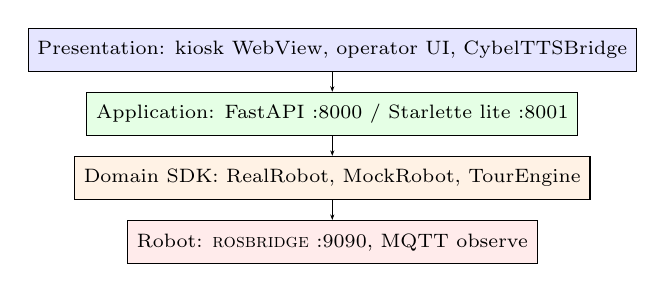
\begin{tikzpicture}[
  layer/.style={draw, minimum width=3.4cm, minimum height=0.55cm, align=center, font=\scriptsize},
  arr/.style={-{Stealth[length=2pt]}}
]
  \node[layer, fill=blue!10] (ui) {Presentation: kiosk WebView, operator UI, CybelTTSBridge};
  \node[layer, fill=green!10, below=0.25cm of ui] (api) {Application: FastAPI :8000 / Starlette lite :8001};
  \node[layer, fill=orange!10, below=0.25cm of api] (sdk) {Domain SDK: RealRobot, MockRobot, TourEngine};
  \node[layer, fill=red!8, below=0.25cm of sdk] (ros) {Robot: \rosbridge{} :9090, MQTT observe};
  \draw[arr] (ui) -- (api); \draw[arr] (api) -- (sdk); \draw[arr] (sdk) -- (ros);
\end{tikzpicture}%
}
\caption{Logical architecture (edge-first, no vendor cloud).}
\label{fig:layers}
\end{figure}

\textbf{Presentation:} \texttt{frontend-kiosk/} visitor UI; \texttt{CybelVisitorKioskTest} APK wraps WebView; \texttt{CybelTTSBridge} handles speech.

\textbf{Application:} FastAPI on PC (port~8000) for development; Starlette \texttt{cybel\_lite.py} on Termux (port~8001 for POI variant) for standalone kiosk without PC.

\textbf{Domain:} \texttt{RobotBackend} protocol with \texttt{MockRobot}/\texttt{RealRobot} implementations --- 83 unit tests pass without physical robot.

\subsection{Edge deployment pattern}

Termux on the tablet runs Python, serves the kiosk over \texttt{0.0.0.0:8001}, connects to \texttt{192.168.20.22:9090}, and triggers TTS via local \texttt{am broadcast}.
The visitor session requires no PC after deployment (\texttt{deploy\_termux.py} or ADB bundle).

%==============================================================================
\section{Conversational Layer Without Vendor Support}
%==============================================================================

The vendor \texttt{welcomepatrol} app couples Iflytek TTS via opaque IPC and a proprietary cloud knowledge API.
\cybel{} replaces this with an \emph{open edge conversational pipeline}:

\begin{enumerate}[leftmargin=1.2em]
\item \textbf{Input:} kiosk touch, operator text, or browser Web Speech API (PC only).
\item \textbf{KnowledgeEngine:} keyword scoring over local JSON (\texttt{knowledgeV2-labV2.json}, FAQ) --- threshold ${\geq}2.0$; deterministic, offline-capable.
\item \textbf{ReceptionService:} matched answer $\rightarrow$ \texttt{RobotSpeech.speak()} + optional \texttt{navigate\_to\_point()}.
\item \textbf{TourEngine:} ordered stops from \texttt{lab\_tour.json} with speech/navigation ordering fix (relocalize \emph{before} TTS to avoid ``speaks but does not move'').
\end{enumerate}

\subsection{TTS channel discovery}

No \ros{} topic, service, HTTP port, or MQTT payload exposed TTS on TY1251D (Table~\ref{tab:tts})~\cite{cybel_tts}.

\begin{table}[!t]
\caption{TTS investigation summary}
\label{tab:tts}
\centering
\scriptsize
\begin{tabular}{@{}ll@{}}
\toprule
\textbf{Channel tested} & \textbf{Result} \\
\midrule
\ros{} publish topics & No subscribers \\
\ros{} services & Absent in \rosapi{} \\
HTTP head (80, 8080, 8888) & Closed \\
MQTT & Odometry only \\
\textbf{ADB broadcast} & \textbf{Working (CybelTTSBridge)} \\
\bottomrule
\end{tabular}
\end{table}

\textbf{CybelTTSBridge} (${\sim}50$\,KB APK): \texttt{BroadcastReceiver} $\rightarrow$ Android \texttt{TextToSpeech} (Google engine, French locale):
\begin{footnotesize}
\begin{verbatim}
am broadcast -n com.cybel.ttsbridge/.SpeakReceiver
  -a com.cybel.ttsbridge.SPEAK --es text "Welcome."
\end{verbatim}
\end{footnotesize}

\texttt{RobotSpeech} tries ROS, HTTP, ADB-from-PC, then local Termux broadcast --- documented fallback chain in \texttt{sdk/speech.py}.

\textbf{LLM extensibility:} \texttt{POST /api/knowledge/ask} accepts the same contract; an LLM backend can call validated \cybel{} navigation/speech APIs without rediscovering \ros{}.

%==============================================================================
\section{Hybrid Navigation Case Study}
%==============================================================================

\subsection{Coordinate-only failure (strategy S1)}

Publishing \texttt{/navi\_goal} with coordinates from a JSON knowledge base often failed in the field: robot spoke but \texttt{nav\_status} remained 601 (planner never entered 602), wrong destinations due to map drift, slow relocalization.

Tour trace \texttt{tour\_20260623\_142601}: goal published, no 601$\rightarrow$602 transition.

\subsection{Sentrymove POI reuse (strategy S3)}

Sentrymove (Deployment Tool) navigates reliably via named POIs on map \texttt{laboV2}.
\cybel{} hybrid flow:
\begin{enumerate}[leftmargin=1.2em]
\item Create POIs in Deployment Tool (\texttt{MAJUSCULES-TIRETS} naming).
\item Sync ROS markers $\rightarrow$ \texttt{data/points.json} (\texttt{sdk/poi\_sync.py}).
\item Kiosk auto-sync on destination grid load; tour uses \texttt{target\_point} in \texttt{lab\_tour.json}.
\item A/B test: port~8000 (coordinates) vs.\ 8001 (POI) on same hardware.
\end{enumerate}

Gap analysis~\cite{cybel_gap} drove fixes: mux teleop topic, POI service chain in lite backend, localization threshold 60\%, cancellation parity.

%==============================================================================
\section{Evaluation and Discussion}
%==============================================================================

\subsection{Metrics (June 2026, lab robot)}

\begin{table}[!t]
\caption{Observed performance indicators}
\label{tab:metrics}
\centering
\scriptsize
\begin{tabular}{@{}ll@{}}
\toprule
\textbf{Metric} & \textbf{Value} \\
\midrule
Local REST latency & ${<}100$\,ms \\
\rosbridge{} connect & 2--60\,s (3$\times$20\,s retry) \\
Session reliability & ${\sim}90\%$ (Wi-Fi dependent) \\
Wi-Fi RTT & 89--1654\,ms \\
Unit tests & 83/83 passed \\
Coord.\ navigation reliability & Low (motivates POI pivot) \\
Termux kiosk autonomously & Validated \\
\bottomrule
\end{tabular}
\end{table}

Validation script: \texttt{phase0\_robot\_check.py --host 192.168.20.22 --teleop --nav-poi "CNC ROUTEUR" --tts}.

\subsection{Lessons for closed robot integration}

\begin{itemize}
\item \textbf{Transport lies:} \rosbridge{} accepts publishes without motor effect; telemetry is ground truth.
\item \textbf{Vendor APK as spec:} JADX of Sentrymove accelerated discovery vs.\ generic \ros{} docs.
\item \textbf{Dual-IP is normal:} document head vs.\ chassis addresses explicitly.
\item \textbf{Reuse over reimplement:} hybrid POI avoids replicating \texttt{marker\_manager}.
\item \textbf{Edge first:} closed robot Wi-Fi precludes cloud LLM/TTS dependencies.
\end{itemize}

\subsection{Limitations}

Chassis shell inaccessible; no native \ros{} TTS; Android~7.1 WebView constraints; DHCP head IP variability; on-robot ASR not yet implemented; ethical APK decompilation for interoperability only.

%==============================================================================
\section{Conclusion}
%==============================================================================

We presented non-destructive reverse engineering of the CIOT TY1251D-03195 and the open \cybel{} platform: seven-phase methodology, validated \rosbridge{} reconstruction, edge architecture with mock/real SDK, Android TTS bridge, local conversational layer, and hybrid Sentrymove POI navigation.

Future work: LLM/RAG behind \texttt{/api/knowledge/ask}, on-device ASR, presence-triggered kiosk wake-up (\texttt{/detected\_people\_array}), and publication of exploration scripts as reproducible artifacts for similar closed Android--\ros{} robots.

%==============================================================================
\section*{Acknowledgment}
%==============================================================================

This work was conducted at HESTIM Engineering \& Business School under supervision of Dr.~Sridath Tula.
We thank the HESTIM robotics lab for robot access and field testing support.

%==============================================================================
\nocite{quigley2009ros,thrun2005probrob,bartneck2020hri,cybel2026}
\bibliographystyle{IEEEtran}
\bibliography{references}

\end{document}
